\documentclass{article}

\usepackage{fancyhdr}
\usepackage{extramarks}
\usepackage{amsmath}
\usepackage{amsthm}
\usepackage{amsfonts}
\usepackage{tikz}
\usepackage[plain]{algorithm}
\usepackage{algpseudocode}

\usetikzlibrary{automata,positioning}

%
% Basic Document Settings
%

\topmargin=-0.45in
\evensidemargin=0in
\oddsidemargin=0in
\textwidth=6.5in
\textheight=9.0in
\headsep=0.25in

\linespread{2.0}

\pagestyle{fancy}
\lhead{\hmwkAuthorName}
\chead{\hmwkClass\ (\hmwkClassInstructor\ \hmwkClassTime)}
\rhead{\firstxmark}
\lfoot{\lastxmark}
\cfoot{\thepage}

\renewcommand\headrulewidth{0.4pt}
\renewcommand\footrulewidth{0.4pt}

\setlength\parindent{0pt}

%
% Create Problem Sections
%

\newcommand{\enterProblemHeader}[1]{
    \nobreak\extramarks{}{Problem \arabic{#1} continued on next page\ldots}\nobreak{}
    \nobreak\extramarks{Problem \arabic{#1} (continued)}{Problem \arabic{#1} continued on next page\ldots}\nobreak{}
}

\newcommand{\exitProblemHeader}[1]{
    \nobreak\extramarks{Problem \arabic{#1} (continued)}{Problem \arabic{#1} continued on next page\ldots}\nobreak{}
    \stepcounter{#1}
    \nobreak\extramarks{Problem \arabic{#1}}{}\nobreak{}
}

\setcounter{secnumdepth}{0}
\newcounter{partCounter}
\newcounter{homeworkProblemCounter}
\setcounter{homeworkProblemCounter}{1}
\nobreak\extramarks{Problem \arabic{homeworkProblemCounter}}{}\nobreak{}

%
% Homework Problem Environment
%
% This environment takes an optional argument. When given, it will adjust the
% problem counter. This is useful for when the problems given for your
% assignment aren't sequential. See the last 3 problems of this template for an
% example.
%
\newenvironment{homeworkProblem}[1][-1]{
    \ifnum#1>0
        \setcounter{homeworkProblemCounter}{#1}
    \fi
    \section{Problem \arabic{homeworkProblemCounter}}
    \setcounter{partCounter}{1}
    \enterProblemHeader{homeworkProblemCounter}
}{
    \exitProblemHeader{homeworkProblemCounter}
}

%
% Homework Details
%   - Title
%   - Due date
%   - Class
%   - Section/Time
%   - Instructor
%   - Author
%

\newcommand{\hmwkTitle}{Homework\ \#8}
\newcommand{\hmwkDueDate}{October 30th, 2015}
\newcommand{\hmwkClass}{Differential Equation}
\newcommand{\hmwkClassTime}{Section 061}
\newcommand{\hmwkClassInstructor}{Professor Heather Lee}
\newcommand{\hmwkAuthorName}{Yao Xiao}

%
% Title Page
%

\title{
    \vspace{2in}
    \textmd{\textbf{\hmwkClass:\ \hmwkTitle}}\\
    \normalsize\vspace{0.1in}\small{Due\ on\ \hmwkDueDate\ at 3:10pm}\\
    \vspace{0.1in}\large{\textit{\hmwkClassInstructor\ \hmwkClassTime}}
    \vspace{3in}
}

\author{\textbf{\hmwkAuthorName}}
\date{}

\renewcommand{\part}[1]{\textbf{\large Part \Alph{partCounter}}\stepcounter{partCounter}\\}

%
% Various Helper Commands
%

% Useful for algorithms
\newcommand{\alg}[1]{\textsc{\bfseries \footnotesize #1}}

% For derivatives
\newcommand{\deriv}[1]{\frac{\mathrm{d}}{\mathrm{d}x} (#1)}

% For partial derivatives
\newcommand{\pderiv}[2]{\frac{\partial}{\partial #1} (#2)}

% Integral dx
\newcommand{\dx}{\mathrm{d}x}

% Alias for the Solution section header
\newcommand{\solution}{\textbf{\large Solution}}

% Probability commands: Expectation, Variance, Covariance, Bias
\newcommand{\E}{\mathrm{E}}
\newcommand{\Var}{\mathrm{Var}}
\newcommand{\Cov}{\mathrm{Cov}}
\newcommand{\Bias}{\mathrm{Bias}}

\begin{document}

\maketitle

\pagebreak


\begin{homeworkProblem}
\subsection{3.8}

(a)We can get 
\[
	u''+256u=0 
\]
So \[
	y=Acos(16t)+Bsin(16t)
\]
Comparing the equation and the 
\( mu''+ku=F_0coswt\)
We get \( w_0=16\)
So the equation becomes
\[
u=Acosw_0t+Bsinw_0t+\frac{F_0}{m(w^2_0-w^2)}coswt 
\]\\
\[ =Acos(16t)+Bsin(16t)+\frac{16}{247}cos(3t) \]
Plug it in with initial condition, we get
\[
 u=\frac{151}{1482}	cos16t+ \frac{16}{247} cos3t
\]
(b) Also we get the plot \\
(c) 
The equation becomes
\[
	 mu''+ku=4sinwt
\]
And we can get
\[
u(t)=Acos(16t)+Bsin(16t)+U(t)
\]
Since \[ U(t)= \frac{32}{256-w^2}sinwt\]
\[ w=w_0=16 \]

\end{homeworkProblem}

\begin{homeworkProblem}
\subsection{Problem k}
\textbf{(a)}

\[y''''=-24 \]
\[y(0)=y(4)=0 \]
\[y'(0)=y'(4)=0 \]
Hence,
\[
\begin{split}
y''''=-24\\
y'''=-24x+Y(x)... \\
y''=-12x^2+Y(x)... \\
y'=-4x^3+Y(x)... \\
y=-x^4+C_1x^3+C_2x^2+C_3x+C_4... \\
\end{split}
\]
Plug it in with the IV, we get
\[
y=-x^4+8x^3-16x^2
\]

\textbf{(b)}
\[
\begin{split}
y'&=(-(-4+x)^2 x^2)'\\
&=-4x(x^2-6x+8)\\
&=-4x(x-2)(x-4)\\
\end{split}
\]
So x=2 or x=4, but when x=4 \(y''<0\) and when x=2 \(y''>0\). The result should be x=2, which is 
\[
x=\frac{L}{2}
\]



\end{homeworkProblem}
\begin{homeworkProblem}
\subsection{Project B}
I use the code below
\begin{verbatim}
function xp=F(t,x)
xp=zeros(2,1); % since output must be a column vector
w=0.1;
xp(1)=x(2);
xp(2)=10*cos(w*t)-4*x(2)-5*x(1);
 
[t,x]=ode45('F',[0,80],[0,0]); plot(t,x(:,1))
\end{verbatim}
The plot below shows the result of \(w=0,0.5,1,2,4,8,16\) accordingly.


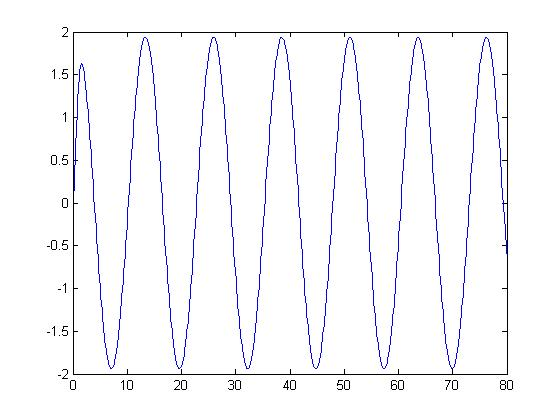
\includegraphics[scale=0.7]{10.jpg}\\
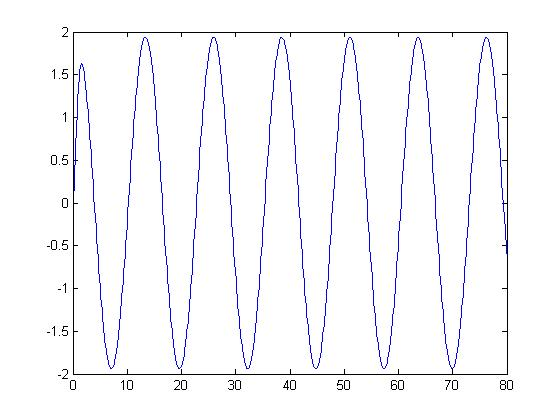
\includegraphics[scale=0.7]{105.jpg}\\
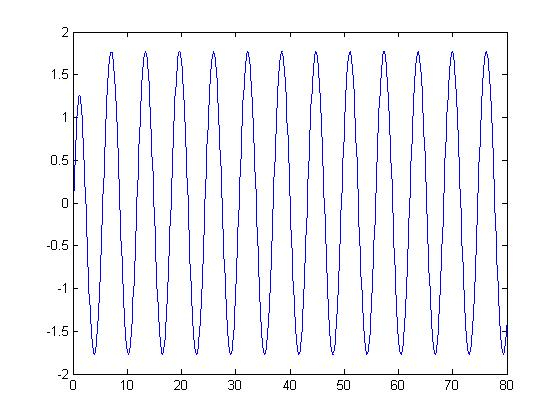
\includegraphics[scale=0.7]{11.jpg}\\
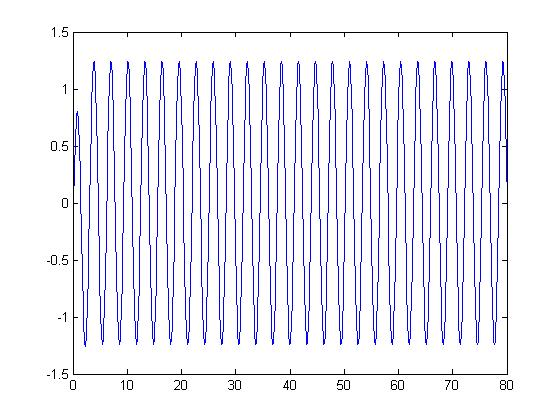
\includegraphics[scale=0.7]{12.jpg}\\
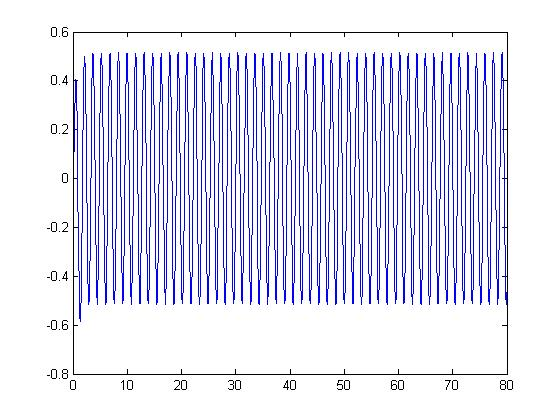
\includegraphics[scale=0.7]{14.jpg}\\
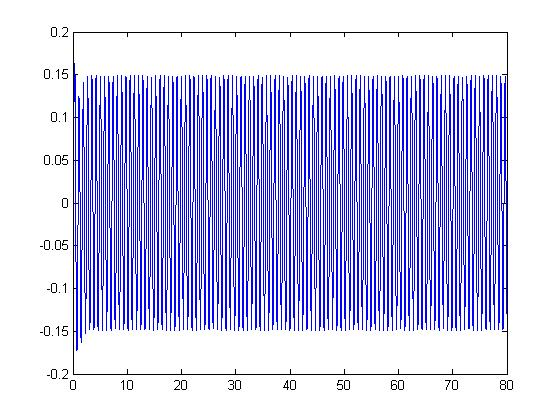
\includegraphics[scale=0.7]{18.jpg}\\
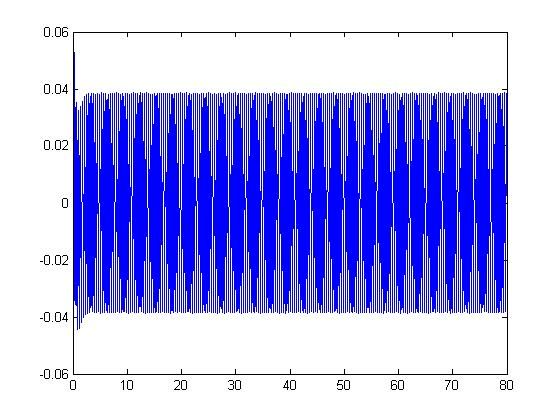
\includegraphics[scale=0.7]{116.jpg}\\

\textbf{(b)}
As state above. I tried \(w=999\) and \(w=0.01\)

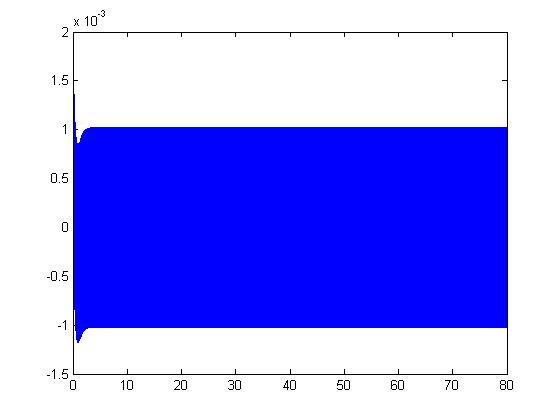
\includegraphics[scale=0.7]{2max.jpg}\\
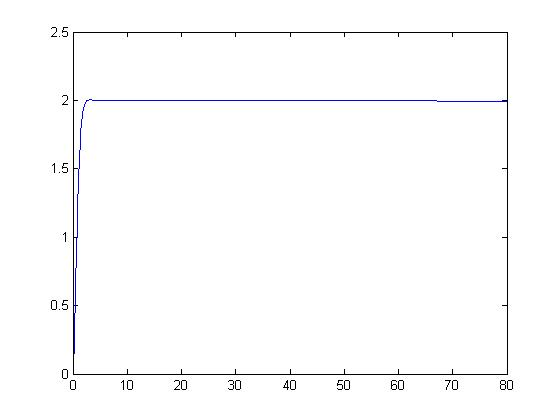
\includegraphics[scale=0.7]{2little.jpg}\\

(The matlab actually broke several times)
From the graph we could draw to the conclusion that as \(w \to \infty \) the \( A(w) \) (which is maximum Displacement) is getting smaller \\
As \(w \to  0 \) the \( A(w) \) (which is maximum Displacement) is getting bigger.



\end{homeworkProblem}


\end{document}
